\documentclass{article}
\usepackage{graphicx}

\title{An example of mosquito evolution in Africa}
\author{Andy Wilkins}

  
\begin{document}
\maketitle

\section{Introduction}

I describe a simple simulation, mainly as an example of the type of simulation that the code can perform.

\section{The spatial domain}

The spatial domain is defined by a $5$\,km$\times 5$\,km grid with lower-left corner at $(x,y)=(-4614,-3967)$ (km) and $n_{x}=1517$ and $n_{y}=1667$, that is
\begin{verbatim}
Grid(-4614.0, -3967.0, 5.0, 1517, 1667, False)
\end{verbatim}
The inactive cells are defined to be those in the ocean, while everything else is active.  This results in $1.4\times 10^{6}$ cells, as shown in Figure~\ref{active_inactive.fig}.

\begin{figure}[htb]
  \centering
  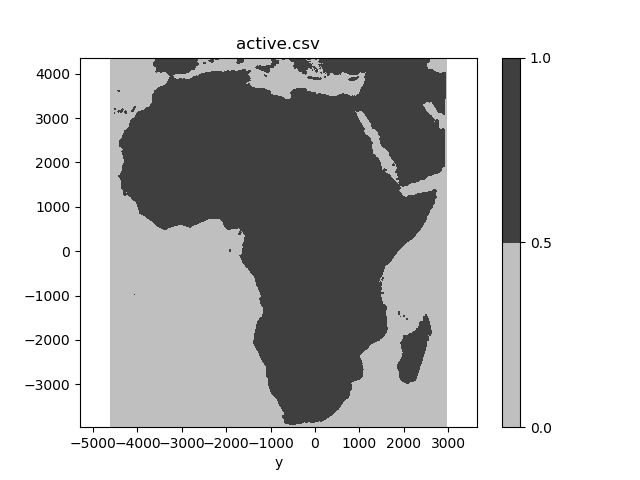
\includegraphics[width=9cm]{active.png}
  \caption{\label{active_inactive.fig}The spatial domain.  Active cells are dark-coloured.}
\end{figure}


\section{Cell dynamics}

The {\tt CellDynamicsLogistic1\_1} class is used.  This solves the logistic equation
\begin{equation}
  \frac{{\mathrm d}P}{{\mathrm d}t} = rP\left(1 - \frac{P}{K}\right) \ ,
\end{equation}
for population $P(t)$.  Here $K$ is the carrying capacity, which varies spatially, and $r$ is a growth rate, defined to be $r=0.1$.day$^{-1}$ for all cells and all times.  This means there is just one population and one parameter (carrying capacity) per cell.  The population, $P$, is assumed to diffuse and advect.

The logistic growth only occurs for 0.5 days out of each day.

\section{Carrying capacity}

This is spatially varying, but is assumed to be constant in time.  It is shown in Figure~\ref{carrying.fig}

\begin{figure}[htb]
  \centering
  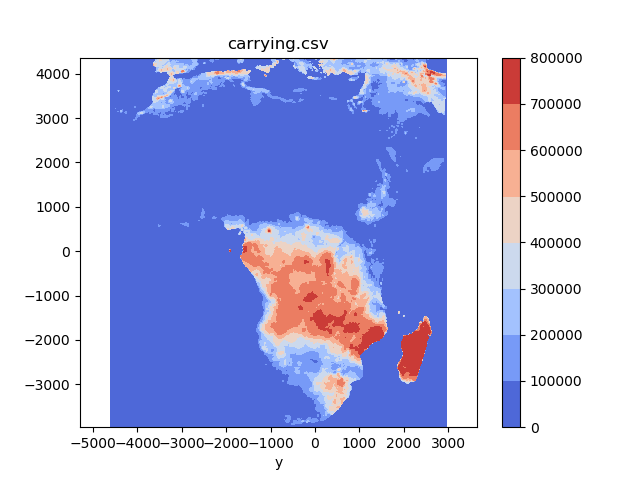
\includegraphics[width=9cm]{carrying.png}
  \caption{\label{carrying.fig}$\log_{10}(\mbox{carrying capacity})$ (mosquitoes per grid cell).}
\end{figure}

\section{Diffusion}

Diffusion is assumed to have a constant, uniform diffusion coefficient of $0.1$\,km$^{2}$.day$^{-1}$.

\section{Advection by wind}

Just one wind file is used, so wind is spatially-varying but temporally constant throughout the simulation.  It is assumed that 1\% of the population, $P$, of each cell enters the wind steam every day.

The probability distribution for mosquitoes to ``drop out'' of the wind stream is assumed to be exponential:
\begin{equation}
  p(t) \propto \left\{
  \begin{array}{ll}
    e^{-6t} & \ \ \mbox{for } t \leq 0.5 \\
    0 & \ \ \mbox{for } t > 0.5
  \end{array}
  \right.
\end{equation}
where $t$ is measured in days.  This gives $p(0)\approx 15$\% and $p(0.5) \approx 0.7$\%.  Hence, regardless of the time-step size, mosquitoes advect for up to 0.5 days every time step.

\section{Initial conditions}

It is assumed that initially there are zero mosquitoes everywhere, except for at cell $(x, y) = (-2000, 700)$, which is in the south of Nigera.  At this cell 10,000 mosquitoes are introduced.  The carrying capacity of the cell is 150,000.  This is shown in Figure~\ref{zoom_0.fig}.

\begin{figure}[htb]
  \centering
  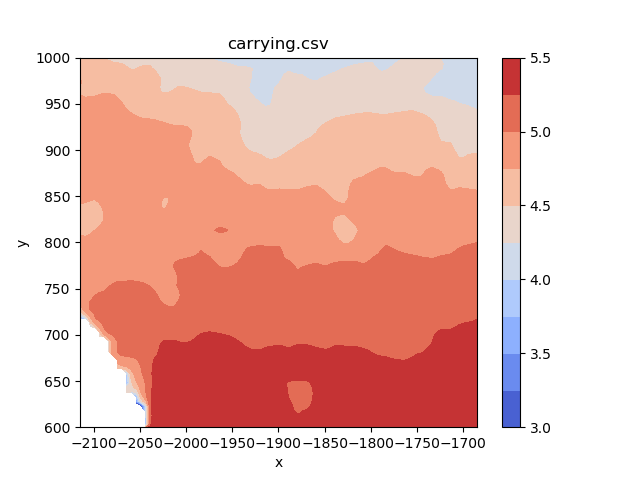
\includegraphics[width=5cm]{carrying_zoom.png} \quad
  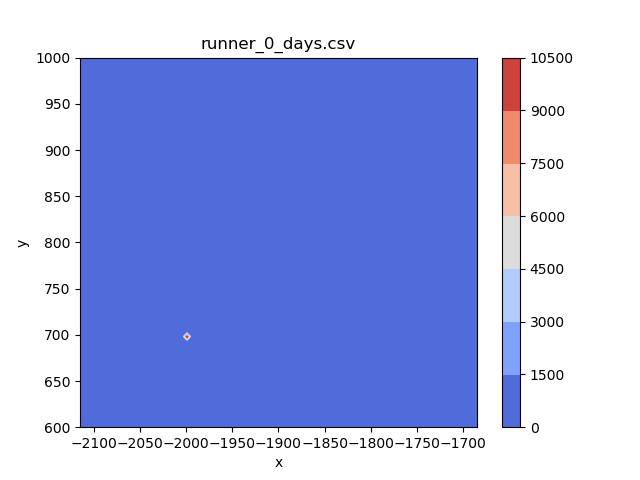
\includegraphics[width=5cm]{runner_0_days.png}
  \caption{\label{zoom_0.fig}Zoomed views into the region of interest.  Left: $\log_{10}(\mbox{carrying capacity})$.  Right: the initial population.}
\end{figure}

\section{Simulation results}

Simulations of 500 days were performed.  No seasonality was included (all parameters are uniform in time).  Two simulations were run: one with wind, and one without wind.  The simulation with wind took 110\,s on my macbook air, and without wind 60\,s.

\begin{figure}[p]
  \centering
  \begin{tabular}{cc}
    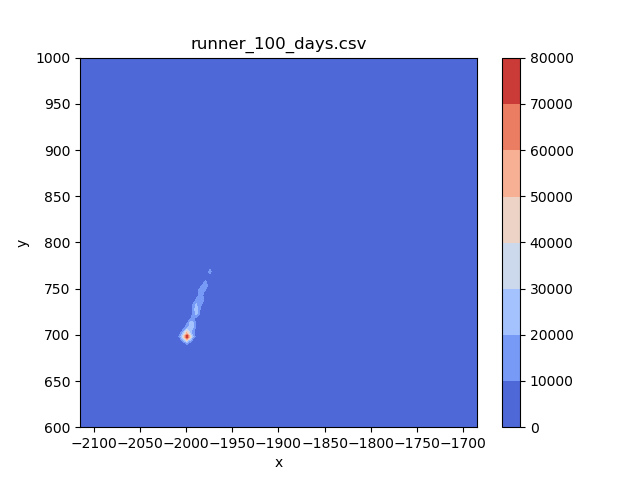
\includegraphics[width=5cm]{runner_100_days.png} &
    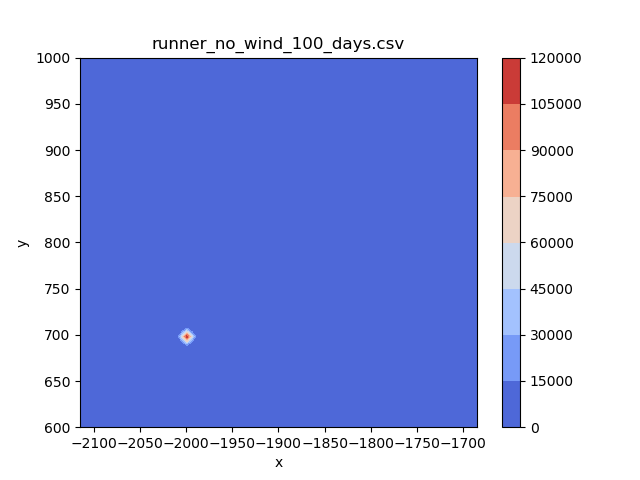
\includegraphics[width=5cm]{runner_no_wind_100_days.png}
    \\
    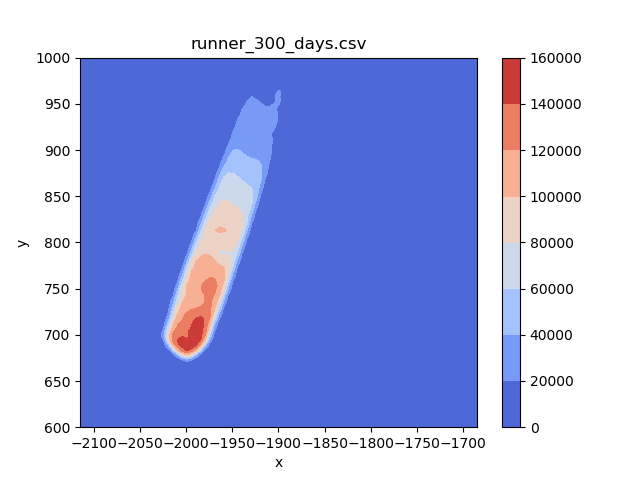
\includegraphics[width=5cm]{runner_300_days.png} &
    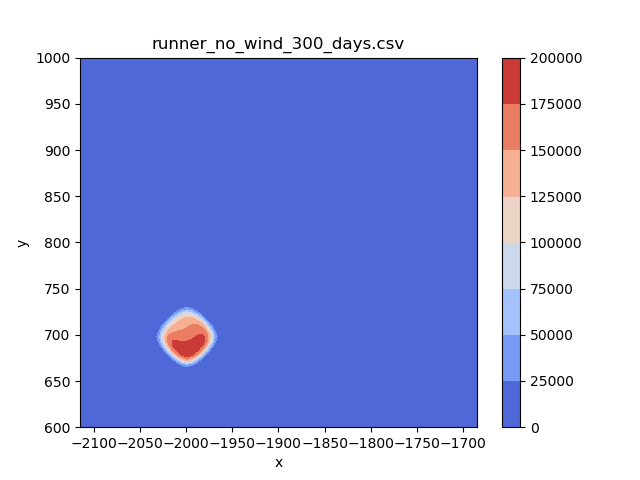
\includegraphics[width=5cm]{runner_no_wind_300_days.png}
    \\
    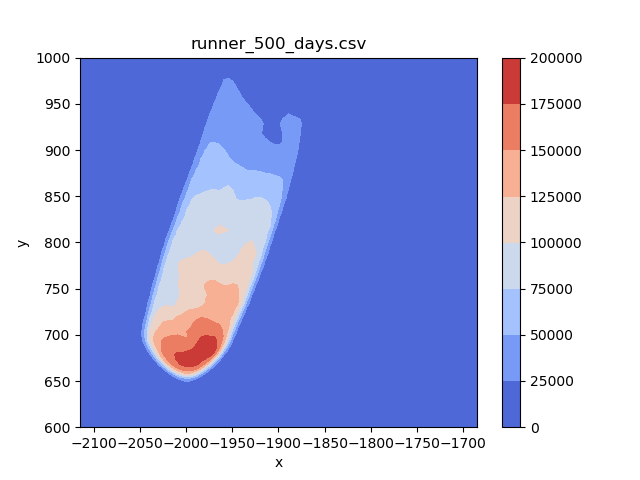
\includegraphics[width=5cm]{runner_500_days.png} &
    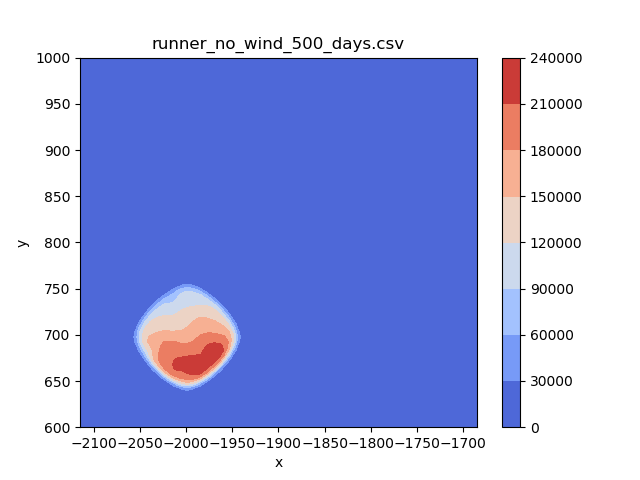
\includegraphics[width=5cm]{runner_no_wind_500_days.png}
  \end{tabular}
  \caption{\label{results.fig}Population results from the simulations.  Left column: with wind.  Right column: without wind.  Notice the colour scales are slightly different in each figure.}
\end{figure}
    






  






\end{document}
